\documentclass[dvips,ruledheader]{abnt}			% header estilo 'plainheader' com uma linha inferior
% \documentclass[dvips,plainheader]{abnt}			% padrão de header da abnt
\usepackage[brazil]{babel} 					% linguagem portugues-Br
\usepackage[T1]{fontenc}
% \usepackage[latin1]{inputenc}
\usepackage[utf8]{inputenc} 					% para aceitar ascentos
\usepackage[pdftex]{graphicx}
% \usepackage[pdftex]{hyperref}
% \usepackage{hyperref}						% incluir links para web
\usepackage{abnt-alf}
\usepackage{latexsym}
\usepackage{psfrag}
\usepackage{epigraph}

% Glossário não utilizado
% \usepackage{makeglo}
% \renewcommand{\glossaryname}{Glossário}
% \makeglossary

\begin{document}
\DeclareGraphicsRule{.eps.gz}{eps}{.eps.bb}{`gunzip -c #1}

% \begin{figure}[topo]
%   \centering
%   \includegraphics[scale=0.3\textwidth]{figuras/}
%   \label{fig:comporte}
% \end{figure}

\autor{Marcio Fernandes Justino}
\titulo{Estudos Gerais de Computação e Forense Computacional para Especialização}
% \orientador[alternativa para ‘Orientador:’ ]{nome do orientador }
% \coorientador[alternativa para ‘Co-orientador:’ ]{nome do co-orientador }
\comentario{Estudo de hardware, software, funcionamento, modus operandi, legislação entre outros conhecimentos necessários para se especializar em computação forense.}
% \instituicao{}
\local{São Bernardo do Campo -- SP}
\data{\today\par\LaTeX{}}

\capa
\folhaderosto

\tableofcontents

\part{Processador}
\chapter{O Papel do Processador}

\part{Discos Rígidos - HDs}
\chapter{Funcionamento dos Discos Rígidos}

\section{Componentes de Funcionamento}

Os discos são guardados em uma espécie de caixa, selada, que evita a entrada de material externo, tendo em vista que uma partícula de poeira pode danificar os discos altamente sensíveis.

\subsection{Discos}

O mercado apresenta tamanhos padrões de HDs, atualmente de 3.5'' para workstations e de 2.5'' para laptops. Há ainda os de 1.8'' e 1'' que são utilizados em dispositivos portáteis como players de áudio. Essas medidas se referem ao diâmetro dos discos.

\subsection{Circuito Lógico}

\subsubsection{Chip Controlador}

O circuito lógico de um HD reúne componentes responsáveis por gerenciar as ações de movimentação dos discos e das cabeças de leitura/gravação, envio e recebimento de dados entre os discos e o computador e rotinas de segurança.

\subsubsection{Chip de Buffer}

Possui a tarefa de armazenar pequenas quantidades de dados durante a comunicação com o computador, utilizado por conseguir trabalhar com os dados em uma velocidade maior que os discos rígidos ele agiliza o processo de transferência de informações.

Atualmente no mercado temos discos com capacidade de buffer entre 2 MB e 64 MB.

\subsection{Pratos e Eixo}

Os pratos são os discos onde os dados são armazenados. Geralmente feitos de alumínio ou um tipo de cristal, recoberto por material magnético e outra camada de material para proteção.

Os HDs de grande quantidade contam com a presença de vários pratos, uns sobre os outros, posicionados sob um eixo que os permite girar. Atualmente eles podem girar a velocidade de 7.200 RPM (rotações por minuto), mas já existem modelos que o fazem a 10.000 RPM. Há pouco tempo atrás o padrão era 5.400 RPM.

\subsection{Cabeça e Braço}

De tamanho bastante reduzido, contém uma bobina que utiliza impulsos magnéticos para manipular as moléculas da superfície dos pratos (discos) e assim realizar a gravação das informações nos mesmos. Há uma cabeça para cada lado do disco. Essa cabeça está posicionada na ponta de um dispositivo chamado \textbf{braço}. Sua função é posicionar as cabeças de leitura/escrita sobre a superfície dos discos.

As cabeças de leitura \textbf{não} tocam os discos fisicamente. A distância é extremamente pequena e a comunicação entre eles é feita pelos impulsos magnéticos já citados.

Em HDs atuais, o cabeçote (que contém as cabeças de gravação/leitura) contém uma cabeça para gravação e outra para leitura separadamente. Em dispositivos mais antigos isso era feito por um único componente.

\subsection{Atuador}

É o componente responsável por mover o braço acima da superfície dos discos, alcançando assim as áreas do disco para realizar as operações de leitura e gravação. O atuador possui uma bobina induzida por imãs que possibilita sua movimentação.

\section{Gravação e Leitura dos Dados}

A superfície dos pratos é composta por materiais sensíveis ao magnetismo (normalmente é utilizado óxido de ferro). O cabeçote manipula as moléculas deste material por meio de seus polos. Para isso, a polaridade das cabeças muda em uma frequência muito alta - quando está positiva, atrai o polo negativo das moléculas e vice-versa. De acordo com esta polaridade é que os bits (0 e 1) são gravados.

No processo de leitura dos dados o cabeçote efetua a leitura do campo magnético gerado pelas moléculas e gera uma corrente elétrica correspondente, cuja variação é analisada pelo controlador do HD para determinar os que foi lido.

\subsection{Organização dos Dados}

Para ordenar os dados é utilizado um esquema conhecido como ``\emph{geometria dos discos}''. Assim, o disco é divido em \textbf{cilindros}, \textbf{trilhas} e \textbf{setores}, como mostra a imagem \ref{fig:disco_divisao}.

\begin{figure}[htb]
\centering
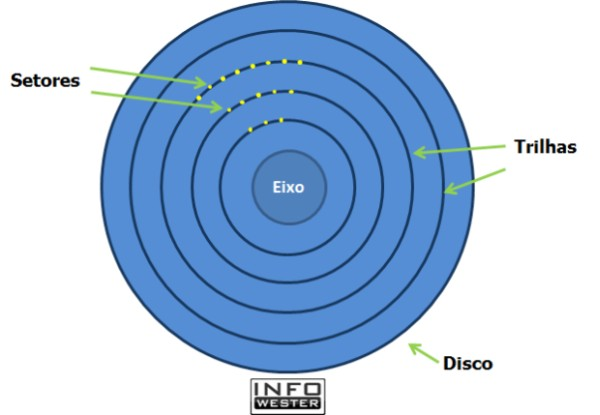
\includegraphics[width=0.8\textwidth]{hd/fig/disco_divisao.png}
\caption{Geometria dos discos}
\label{fig:disco_divisao}
\end{figure}

\subsubsection{Trilhas e Setores}

As trilhas são raios ao redor do eixo do disco que começam em sua borda e vão até o centro. Essas trilhas são numeradas a partir da borda do disco começando pela trilha 0. Cada trilha é dividida em trechos regulares chamados de setores. Cada setor possui uma capacidade determinada de armazenamento (geralmente, 512 bytes).

\subsubsection{Cilindros}

Sabe-se que o HD possui vários pratos e que há uma cabeça de leitura de gravação de cada lado do disco, e que há somente um braço de leitura para todos os discos e que se movimenta igualmente para todos os discos, quando se quer ler uma determinada trilha de um dos discos, automaticamente o cabeçote se posiciona nessa mesma trilha em todos os discos. Quando isso ocorre dá-se o nome de cilindro\footnote{Cilindro é a posição das cabeças de leitura/gravação sobre as mesmas trilhas de seus respectivos discos.}.

\subsubsection{Formatação}

Para receber os dados o disco precisa estar ``preparado''. Essa preparação é feita através da formatação. Há 2 tipos de formatação:

\begin{itemize}
	\item Física; e
	\item Lógica.
\end{itemize}

\textbf{Física}

A formatação física é a divisão do disco nas estruturas de tricas e setores. Esse procedimento é feito pelo fabricante do HD obedecendo os padrões estabelecidos.

\textbf{Lógica}

Por sua vez, esta formatação consiste na aplicação de um sistema de arquivos apropriado para cada sistema operacional. O Windows, por exemplo, é capas de trabalhar com sistemas FAT e NTFS, já o linux é capaz de trabalhar com vários sistemas de arquivos, dentre eles o ext3 e o ReiserFS.

\section{Interfaces de Comunicação}

Para se comunicar com o computador, o HD utiliza uma interface capaz de transmitir os dados entre ele e o computador de maneira segura e eficiente.

Os padrões de interface mais comuns são:

\begin{itemize}
	\item IDE;
	\item SCSI; e
	\item SATA.
\end{itemize}

\subsection{IDE(PATA)}

A interface IDE, também conhecida como \emph{\textbf{ATA}}, ligação feita através de um cabo flat (\emph{flat cable}) de 40 vias, posteriormente sendo utilizado um cabo de 80 vias cujos fios extras servem para evitar a perda de dados causadas por ruídos (interferências). A imagem \ref{fig:hd_cabo_ide} ilustra um modelo de cabo flat de 80 vias.

\begin{figure}[htb]
  \centering
  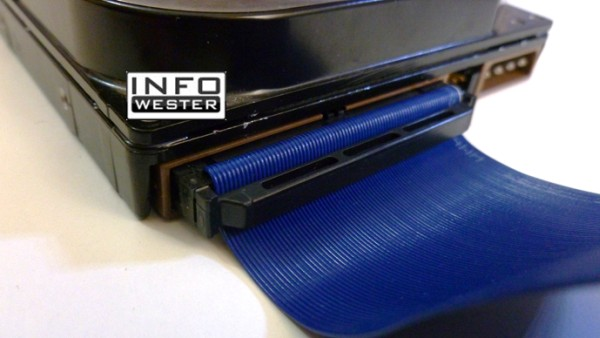
\includegraphics[width=0.8\textwidth]{hd/fig/hd_cabo_ide.jpg}
  \caption{Cabo flat de 80 vias}
  \label{fig:hd_cabo_ide}
\end{figure}

Como com o cabo flat e a conexão IDE é possível se conectar 2 HDs simultaneamente, existe um \emph{jumper} posicionado na traseira do HD que possibilita que o dispositivo (HD) possa ser identificado como sendo ``primário'' ou ``secundário''. Esse é o meio que possibilita que o computador saiba quais dados correspondem a cada dispositivo. A figura \ref{fig:hd_ide} mostra a localização do jumper no HD.

\begin{figure}[htb]
  \centering
  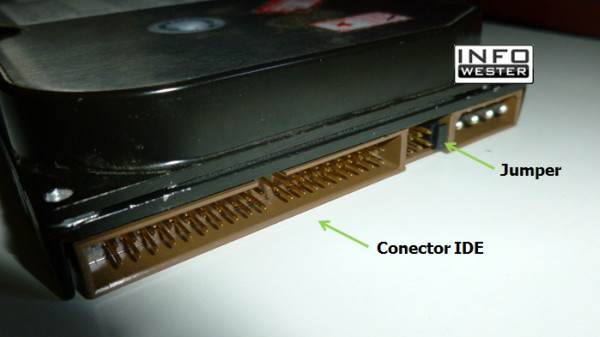
\includegraphics[width=0.8\textwidth]{hd/fig/hd_ide.jpg}
  \caption{Localização do jumper no HD}
  \label{fig:hd_ide}
\end{figure}

\newpage

A interface IDE ainda possibilita a conexão de outros dispositivos como unidades de CD/DVD. Para tal, a IDE utiliza um padrão conhecido como ATAPI que funciona como uma extensão para tornar a IDE compatível com tais dispositivos. A própria BIOS é capaz de reconhecer que tipo de aparelho está conectado em suas entradas IDE e utiliza a tecnologia correspondente (em geral, ATAPI para unidades de CD/DVD e ATA para discos rígidos).

\subsubsection{EIDE}

Uma extensão da interface IDE, possibilita a conexão simultânea de até 2 dispositivos por IDE além de aumentar a velocidade de transmissão de dados dos discos dispositivos.

\subsection{DMA e UDMA}

Antigamente, somente o processador tinha acesso direto aos dados da memória RAM. Com isso se qualquer outro componente do computador precisasse de algum dado da memória, teria que fazer acesso por intermédio do processador.

DMA (Direct Memory Access), como o próprio nome diz, tornou possível o acesso direto à memória pelo HD e outros dispositivos, sem o ``auxílio'' direto do processador.

Quando o DMA não está em uso, normalmente é utilizado um esquema de transferência de dados conhecido como PIO (Programmed I/O), onde o processador executa transferência de dados entre o HD e a memória RAM.

O UDMA permite transferência de dados a uma taxa maior que o DMA, de pelo menos 133 MB/s no caso do UDMA133, e é necessário que o chipset da placa mãe também o suporte, caso contrário, a transferência de dados será reduzida ao suportado pelo chipset da placa mãe.

\subsection{SATA}

Alcance de maiores velocidades na transferência de dados e facilidade de conexão e economia de espaço.

\begin{itemize}
  \item \textbf{SATA I}: até 150 MB/s;
  \item \textbf{SATA II}: até 300 MB/s; e
  \item \textbf{SATA III}: até 600 MB/s.
\end{itemize}

\subsection{SCSI - Small Computer System Interface}

Espercificação antiga, criada para permitir transferências de dados mais rápidas, de até 320 MB/s.

\subsection{NCQ - Native Command Queuing}

Comum nos discos rígidos atuais, o NCQ pode otimizar o desempenho do dispositivo a partir de um esquema de reorganização capaz de diminuir a carga de trabalho da unidade.

Em vez de a cabeça de leitura/gravação seguir pontos em sequência de dados ela segue a leitura conforme a proximidade dos dados, ou seja, se o ponto 3 estiver mais próximo do 1 do que o 2, a sequência de acesso será 1, 3 e 2. A figura \ref{fig:ncq} mostra a comparação de uma leitura de dados em um HD sem NCQ com um outro HD com o uso do NCQ.

\begin{figure}[htb]
  \centering
  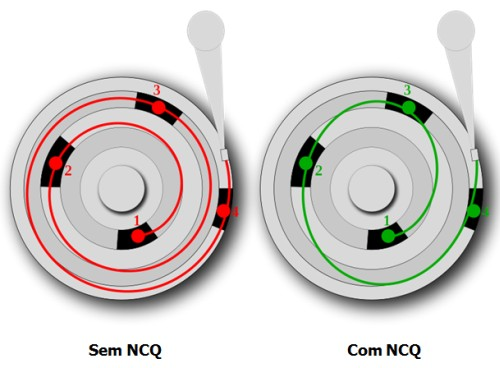
\includegraphics[width=0.8\textwidth]{hd/fig/ncq.jpg}
  \caption[Comparativo]{À esquerda um HD sem NCQ; À direita um HD com NCQ}
  \label{fig:ncq}
\end{figure}


\part{Sistemas de Arquivos}
\chapter{A Estrutura dos Arquivos}

Um arquivo possui a estrutura:

\begin{itemize}
	\item Cabeçalho;
	\item Texto;
	\item Dados;
	\item Bits de relocação; e
	\item Tabela de símbolos.
\end{itemize}

O cabeçalho começa com o número mágico, que identifica o arquivo com executável (para impedir a execução acidental de um arquivo que não seja desse formato). Na sequência vem o tamanho das várias partes do arquivo, o endereço no qual a execução deve iniciar e alguns bits de sinalização. Após o cabeçalho temos o texto e os dados do programa propriamente ditos, que são carregados na memória e relocados usando bits de relocação. A tabela de símbolos é usada para depuração do arquivo.

\section{Atributos de Arquivo}

Todo sistema operacional associa ao arquivo informações como por exemplo:

\begin{itemize}
	\item Data e horário de criação;	
	\item Data e horário de alteração;	
	\item Data e horário de último acesso;
	\item Criador do arquivo;
	\item Proprietário atual do arquivo;
	\item Flag's de controle;
	\item Tamanho do arquivo; e
	\item Proteção do arquivo.
\end{itemize}

Essas informações extras dos arquivos são conhecidas como atributos do arquivo. Esses atributos variam de um sistema para outro. Alguns atributos são alterados pelo sistema operacional quando ocorre alguma interação com o arquivo para que a ação sobre ele possa ser identificada futuramente.

\section{Esquema do Sistema de Arquivos}

Os sistemas de arquivos são armazenados em discos. O setor 0 do disco é chamado de MBR (Master Boot Record - registro de controle de iniciação do sistema) e é usado para iniciar o computador. O final da MBR contém a tabela de partição, que indica os endereços iniciais e finas de cada partição do disco. Uma delas é marcada como ativa, quando o computador é iniciado, a BIOS lê e executa o MBR. Assim, a primeira coisa que a MBR faz é localizar a partição ativa, ser seu primeiro bloco (bloco de boot) e executá-lo. O programa de bloco de boot carrega o sistema operacional contido na partição.

A figura \ref{fig:esquema_sistemas_arquivos} demonstra como, no geral, é estruturado o sistema de arquivos no disco.

\begin{figure}[htb]
	\centering
	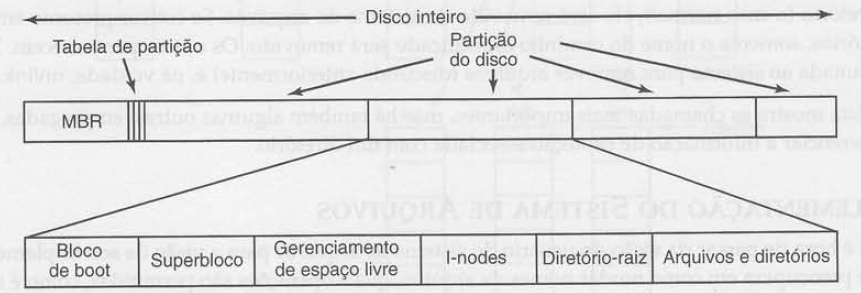
\includegraphics[width=0.8\textwidth]{sistemas_de_arquivos/fig/esquema_sistemas_arquivos.png}
	\caption{Possível layout de sistema de arquivos}
	\label{fig:esquema_sistemas_arquivos}
\end{figure}

\chapter{Capacidade de Armazenamento}

Vimos que a geometria do disco rígido envolve trilhas, setores e cilindros e que em cada setor do disco cabem 512 bytes de informação. Para identificar a capacidade de armazenamento de um disco basta utilizar a geometria, se um disco tem 2.448 cilindros, 16 lados (ou ``cabeças'' de leitura) e 63 setores por trilha, terá 2.448 x 16 x 63 = 2.467.584 setores. Logo, se multiplicarmos a quantidade de setores pela quantidade de informação que cabe em cada setor teremos a capacidade total do disco, que no caso é de 1.263.403.008 bytes, e como cada KB tem 1.024 bytes, dividindo-se por 1.024 uma vez para identificar a quantidade de KB do disco, divide-se novamente para identificar a quantidade em MB e novamente para identificar a quantidade em GB. Sendo assim esse disco teria a capacidade real de 1.18 GB.

\chapter{FAT}

\section{FAT-16}

O sistema FAT (File Allocation Table), utiliza uma tabela de alocação de arquivos representando um mapa de utilização do disco, o que permite ao sistema operacional ser capaz de saber exatamente onde um determinado arquivo está armazenado.

A FAT possui várias posições para localização de arquivos no disco. Como cada posição na FAT-16 utiliza 16 bits, podemos ter, no máximo, 256 (16 \^ 2) = 65.536 posições na FAT.

\subsection{Tabela de Alocação}

Como em um setor cabem 512 bytes, teoricamente, só poderiamos ter discos de 65.536 x 512 bytes = 33.554.432 bytes = 32 MB. Por esse motivo, o sistema FAT-16 não trabalha com setores mas sim com unidades de alocação chamadas \emph{\textbf{clusters}}, que é um conjunto de setores.

\subsection{Cluster}

Ao invés de cada posição da FAT apontar para um setor, ela aponta para um cluster, podendo ser de 1, 2, 4 ou mais setores do disco. O tamanho do cluster é definido automaticamente pelo sistema operacional quando o disco é formatado, seguindo uma tabela.

Sendo o cluster a menor unidade a ser acessada pelo sistema operacional, os arquivos deverão ter obrigatoriamente tamanhos múltiplos do tamanho do cluster, o que significa que um arquivo de 100 KB em um disco rígido que utilize clusters de 8KB obrigatoriamente ocupará 13 clusters e não 12,5 como seria a divisão de 100 por 8. Isso daria um total de 104 KB, neste caso temos um \emph{\textbf{desperdício}} de 4 KB. Quanto maior o tamanho do cluster, maior o desperdício.

Esse espaço deixado pelo arquivo dentro do cluster é muito importante para a forense computacional, chamado de \textbf{Slack Space}. Esse espaço costuma ficar vestígio de arquivos manipulados no sistema. 

\begin{citacao}
  Forense em sistemas FAT-16 podem apontar grandes quantidades de informações em slack space.
\end{citacao}

Todo o espaço que de armazenamento que sobra de um cluster não é reutilizado para armazenar outro arquivo. \emph{Um cluster só pode ser utilizado por um arquivo.}

Uma limitação do FAT-16 é que ele só permite gerenciar discos de até 2 GB de partição.

\subsection{FAT-32}

Com o FAT-32 o tamanho do cluster é sensivelmente menor, fazendo com que haja bem menos desperdício, reduzindo o slack space. Permite, também, o uso de discos maiores, até 1 TB em uma partição.

\section{NTFS}

Esse sistema de arquivos permite que a menor unidade de alocação (512 bytes) possa ser usada como o próprio setor, evitando assim desperdício de espaço.

O sistema NTFS utiliza 64 bits para endereçar os dados em sua MFT (Master File Table - tabela de endereçamento). Com o uso de clusters de 64 KB o limite de dados pode chegar aos 256 TB. O tamanho do cluster é definido automaticamente pelo sistema operacional ou pela formatação de uma partição, podendo ir de 512 bytes a 64 KB, e também podendo ser definido pelo usuário em procedimentos específicos.

\begin{citacao}
  Durante o processo de formatação do disco, é criado o MBR (Master Boot Record). O MBR contém uma quantidade pequena de códigos executáveis chamada de ``master boot code'' e contém também a tabela de partição do disco. A tabela de partição contém um determinado número de campos para descrever a partição. Um desses campos é o System ID, que define o file system, como o NTFS, na partição. Para volumes NTFS o ID é 0x07. 
\end{citacao}

A figura \ref{fig:ntfs} demonstra a arquitetura do NTFS.

\begin{figure}[htb]
	\centering
	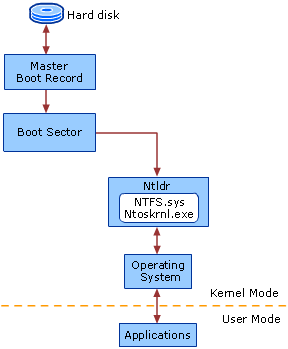
\includegraphics[width=0.8\textwidth]{sistemas_de_arquivos/fig/ntfs.png}
	\caption{Arquitetura do NTFS}
	\label{fig:ntfs}
\end{figure}

\newpage

O link \textbf{http://technet.microsoft.com/en-us/library/cc781134(v=ws.10).aspx} serve como referência para aprofundamento no NTFS.

\subsection{Tolerância a Falhas}

Para preservar os dados o NTFS utiliza um esquema de \emph{journaling}, um arquivo de log que indica falhas para posterior recuperação de dados. O log registra todas as ações que acontecem no sistema em relação aos arquivos. Quando um documento é criado, um espaço é alocado para ele, suas permissões são definidas, e assim por diante. Nesse meio tempo pode haver uma queda de energia e o espaço definido para o arquivo ser alocado, mas não utilizado. Quando o sistema operacional é reativado, ele consulta o arquivo de log para saber quais procedimentos não foram executados por completo e executa a ação correspondente para corrigir o problema.

\subsection{MFT - Master File Table}

A MFT tem praticamente a mesma finalidade da FAT, porém, funciona de uma forma diferente.

O MFT registra atributos de cada arquivo armazenado, consistindo em uma série de informações como por exemplo:

\begin{itemize}
	\item Nome do arquivo;
	\item Data da última modificação;
	\item Permissões; e
	\item Localização na unidade de armazenamento.
\end{itemize}

Cada entrada na MFT possui cerca de 2 KB, onde são armazenados o nome do arquivo e seus atributos, sobrando uma pequena área de dados que é usada para guardar o início do arquivo.

\begin{citacao}
  Em alguns casos, não é possível armazenar nem mesmo os atributos do arquivo, neste caso, os atributos são gravados em clusters no HD e na MFT ficam as entradas que apontam para os clusters.
\end{citacao}

\subsection{EFS}

O EFS é um recurso de criptografia permitindo uma maior proteção dos dados por criptografia utilizando chaves públicas. A principal vantagem é que o dono dos arquivos protegidos pode determinar quais usuários prodem acessá-los.

\subsection{Multiple Data Streams}

NTFS suporta multiplos streams de dados, onde o nome da stream identifica um atributo de dados novo no arquivo. O stream, então, é um conjunto exclusivo de atributos de arquivos. Os streams possuem atributos diferentes como bloqueio de arquivo e tamanho mas, possui \emph{\textbf{permissões comuns}}. 

Esse recurso permite gerenciar os dados com uma única unidade. Exemplo de um stream:

{
\raggedright
myfile.dat:stream2
}

Uma biblioteca de arquivos pode existir onde os arquivos são definidos como streams alternativos, como mostra o exemplo:

{
\raggedright
library:file1
:file2
:file3
}

Um arquivo pode estar associado a mais de uma aplicação ao mesmo tempo, assim como  Microsoft Word e Microsoft WordPad. Um exemplo da estrutura de arquivo que demonstra a associação múltipla a várias aplicações mas não múltiplos arquivos:

{
\raggedright
$
program:source_file
:doc_file
:object_file
:executable_file
$
}

Uma forma de criar um arquivo com stream alternativo:

{
\raggedright
$
echo text > program:source_file
more < program:source_file
$
}

\begin{citacao}
Um detalhe muito importante é que essa funcionalidade está presente somente no NTFS e é incompatível para o FAT, ou seja, se um disco com sistema de arquivo FAT receber a cópia de um arquivo NTFS os streams e outros atributos não suportados pelo FAT serão perdidos sem nenhum aviso.
\end{citacao}

\subsection{Change Journal}

O Change Journal é usado pelo NTFS para prover um log persistente de todas alterações feitas em arquivos no volume. \textbf{Para cada volume}, o NTFS usa o change journal para rastrear informações sobre inclusão, remoção e modificação de arquivos.

fonte: \textbf{http://www.readability.com/articles/xhgmtysq}

\section{EXT3}

Possui o recurso de recuperação de falhas, o \emph{\textbf{Journaling}}. Isso poderia ser relevante para a forense pois alguns dados e metadados registrados na área de ``Journal'' do sistema podem significar alguma coisa em uma investigação, principalmente se utilizando o tipo de trabalho ``Journal''.

\subsection{Journaling}

O ext3 trabalha com 3 diferentes tipos de Journaling:

\begin{itemize}
	\item \textbf{Journal}: grava todas mudanças em sistema de arquivos. É o mais lento dos três modos, mas é o que apresenta maior capacidade de evitar perda de dados;
	\item \textbf{Ordered}: grava somente mudanças em arquivos \emph{metadata} (arquivos que guardam informações de outros arquivos), mas guarda as atualizações no arquivo de dados antes de fazer as mudanças associadas ao sistema de arquivos. Este é o Journaling padrão nos sistemas de arquivos ext3;
	\item \textbf{Writeback}: também só grava mudanças para o sistema de arquivo em \emph{metadata}, mas utiliza o processo de escrita do sistema de arquivos em uso para gravação. É o mais rápido de todos, mas o menos confiável.
\end{itemize}

\subsection{Superbloco}

Registro que descreve as características do sistema de arquivos, conforme a figura \ref{fig:superbloco}.

\begin{figure}
	\centering
	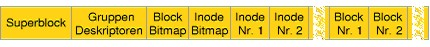
\includegraphics[width=0.8\textwidth]{sistemas_de_arquivos/fig/superbloco.jpg}
	\caption{Informações do superbloco}
	\label{fig:superbloco}
\end{figure}

O superbloco contém informações sobre:

\begin{itemize}
	\item Comprimento de um bloco de disco;
	\item Tamanho e localização das tabelas de i-nodes;
	\item Mapa de blocos de disco e informações sobre utilização; e
	\item Tamanho dos grupos de blocos.
\end{itemize}

O GNU/Linux mantém, para cada sistema de arquivos, um cópia do superbloco em memória RAM. A chamada de sistema ``sync'' despeja os dados sobre os superblocos que estão armazenados em memória cache para seus locais em disco, sincronizando as informações sobre o sistema de arquivos. Essa sincronização torna o sistema de arquivos consistente rapidamente. Essa operação acontece automaticamente em intervalos de 30s para sistemas ext2 e de 5s para sistemas ext3, reduzindo ainda mais a possibilidade de falhas em servidores com intensas atividades de gravação de arquivos.

\begin{citacao}
A destruição do superbloco deixa o sistema de arquivos ilegível.
\end{citacao}

\subsection{i-nodes}

I-nodes são entradas de tabelas de comprimento fixo, cada uma das quais armazenam informações sobre um arquivo existente no sistema de arquivos. Cada i-node tem o tamanho fixo de 64 bytes e descreve exatamente um arquivo. O i-node contém informações suficientes para localizar todos os blocos do disco que contenham os dados do arquivo.

Os dados do arquivo são armazenados em unidades chamadas de ``blocos''. Um arquivo também possui um ``i-node''. Os blocos e os i-nodes são numerados sequencialmente porém, o i-node possui uma sequência diferente da dos blocos. Uma entrada de diretório consiste do nome do arquivo e de um número de i-node. O i-node também armazena o local dos blocos de dados, como pode ser visto na figura \ref{fig:inode} e \ref{fig:inode_esquema}.

\begin{figure}
	\centering
	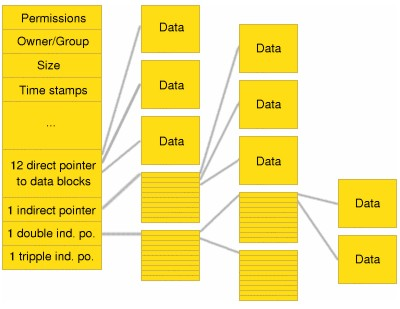
\includegraphics[width=0.8\textwidth]{sistemas_de_arquivos/fig/inode.jpg}
	\caption{Forma como o \emph{inode} armazena o local dos blocos de dados}
	\label{fig:inode}
\end{figure}

\begin{figure}
	\centering
	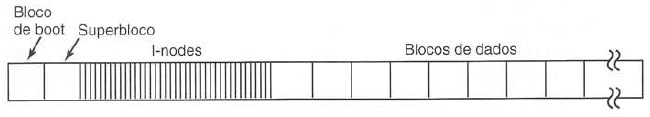
\includegraphics[width=0.8\textwidth]{sistemas_de_arquivos/fig/inode_esquema.jpg}
	\caption{Esquema do disco em sistemas Unix clássicos.}
	\label{fig:inode_esquema}
\end{figure}

\begin{itemize}
	\item Os números dos primeiros 12 blocos são armazenados diretamente no i-node - chamados de ``blocos diretos'' (pode ser visto na figura \ref{fig:inode} em ``12 direct pointer to data blocks'');
	\item O i-node contém o número do bloco de um bloco indireto. (pode ser representado na figura \ref{fig:inode} em ``1 indirect pointer''). Um bloco indireto contém os números de blocos de 256 blocos de dados adicionais;
	\item O i-node contém o número do bloco de um bloco duplamente indireto (pode ser visto na figura \ref{fig:inode} em ``1 double ind. po.''). Um bloco duplamente indireto contém os números de blocos de 256 blocos indiretos adicionais; e
	\item O i-node contém o número do bloco de um bloco três vezes indireto. (pode ser visto na figura \ref{fig:inode} em ``1 tripple ind. po.''). Um bloco três vezes indireto contém os números de blocos de 256 blocos duplamente indiretos adicionais.
\end{itemize}

Sendo assim, o sistema de arquivo ext3 consiste de 5 componentes estruturais.

\begin{itemize}
	\item Células de armazenamento i-node;
	\item Superblocos distribuídos;
	\item Mapa de blocos no sistema de arquivos;
	\item Resumo de emprego de blocos; e
	\item Conjunto de blocos de dados.
\end{itemize}

Cada partição de sistema de arquivos é dividida em grupos de blocos. Estruturas como as tabelas de i-node são alocadas entre os grupos de blocos para que os blocos que são acessados juntos possam ser armazenados próximos uns dos outros no disco.

Os i-nodes são criados no momento da formatação lógica do hd. Assim é possível redimensionar o número de i-nodes de acordo com a capacidade do hd, tipo e tamanho de arquivos que serão armazenados nele. O número de i-nodes não pode ser ajustado após a formatação inicial.

\subsection{Mapa de Blocos}

É a tabela de blocos livres que o disco possui. Quando da gravação de um arquivo novo, esse mapa é verificado de modo que uma disposição eficiente seja utilizada.

\subsection{Blocos de Dados}

Após os i-nodes aparecem os blocos de dados. Neles são armazenados todos os arquivos (e diretórios também). Se um arquivo ou diretório é constituído de mais de um bloco, eles não precisam estar em sequência no disco, pelo contrário, normalmente os blocos de um arquivo grande estão espalhados e dispersos por todo o disco.

\subsection{Resumos de Empregos de Blocos}

Registram informações básicas sobre os blocos que já se encontram em uso.

Até este ponto os sistemas ext2 e ext3 são idênticos.

\section{ReiserFS}

Possui suporte ao ``journaling'' e atualmente presente como padrão para distribuições GNU/Linux da SuSE, Gentoo e Linspire.

Ele trata toda a partição como se fosse uma única tabela de banco de dados contendo diretórios, arquivos e metadados dentro de uma mesma árvore. Essa característica exigiu o uso de técnicas de indexação mais complexas para tornar os tempos de resposta do ReiserFS mais eficientes comparados com outros sistemas de arquivos. O ReiserFS usa uma árvore \textbf{finita} (número de nós é limitado).

O ReiserFS possui suporte a arquivos maiores que 2GB.

ReiserFS usa árvores balanceadas (B*) para tornar o processo de busca de arquivos, informações sobre segurança e outros metadados mais eficientes.

Outra grande vantagem do ReiserFS é a alocação dinâmica de i-nodes, já que esse sistema de arquivos não os aloca em espaços fixos ou blocos e sim, aloca o tamanho exato que o arquivo precisa. Em sistemas baseados em i-nodes fixos, como o EXT3, o espaço no disco é alocado em blocos que variam de 512 a 4096 bytes ou até maior, caso o arquivo exceda um múltiplo exato do tamanho do bloco.

Seu uso de funções hash e árvores balanceadas (B*), ao invés de seqüências infindáveis de i-nodes, tornam a procura de um arquivo em uma dezena ou em uma grande quantidade uma operação bem rápida.

No caso de um desligamento incorreto do sistema, o ReiserFS é capaz de recuperar a consistência do sistema de arquivos em frações de segundo e a possibilidade de perda de pastas ou partições é nula. Em compensação, os arquivos que eventualmente estiverem sendo gravados no exato momento em que acabou a energia ficarão com seus dados alterados. Você continuará tendo acesso aos arquivos normalmente, mas o conteúdo estará truncado ou incompleto.

Fonte: \textbf{http://www.readability.com/articles/euug5xab}



\part{Sistemas Operacionais}
\chapter{O Uso da Memória}

\chapter{O Sistema Operacional}

% \include{introducao}
% \include{objetivo}
% \include{requisito}
% \include{configuracao}
% \include{comportamento}
% \include{utilizacao}
% \include{recuperacao}
% \include{problemas}

% \bibliography{bb}
% \bibliographystyle{abnt-alf}

\end{document}